\subsection{RGB Konvertierung}

Für die Analyse des CMBs werden die sphärischen harmonische Koeffizienten 
$c_l^m$ benötigt. Dafür müssen aber erst die Bilddaten, welche im RGB Format 
vorliegen Kelvin Werte umgewandelt werden. Da nicht klar ist, wie genau die 
Ursprüngliche Transformation aussah, wird die Analyse mittels einer Annäherung 
an die wirkliche Transformationsfunktion durchgeführt.

Den dafür benötigten Referenzfarbverlauf finden wir in den Resultaten der 
Planck Mission \cite{planck_overview}, zu sehen in 
Abbildung~\ref{fig:color-strip-orig}. Ein Blick auf die einzelnen RGB Kanäle 
zeigt, wie die Funktion aussehen könnte (siehe 
Abbildung~\ref{fig:color-strip-orig-rgb}). Da es dabei aber um einen Screenshot 
der im PDF Dokument enthaltenen Grafik handelt, ist nicht anzunehmen, dass die 
Funktion genau so aussieht. Als mögliche Annäherung wird daher der Farbverlauf 
in Abbildung~\ref{fig:color-strip} mit dem RGB Profil in 
Abbildung~\ref{fig:color-strip-rgb} als Transformationsfunktion verwendet.



\begin{figure}
	\centering
	
\includegraphics[width=\linewidth]{cmb/images/color-strip-full.png}
	\caption{Farbverlauf der für die Codierung des CMB Bildes der ESA Planck 
		Mission verwendet wurde.}
	\label{fig:color-strip-orig}
\end{figure}

\begin{figure}
	\centering
	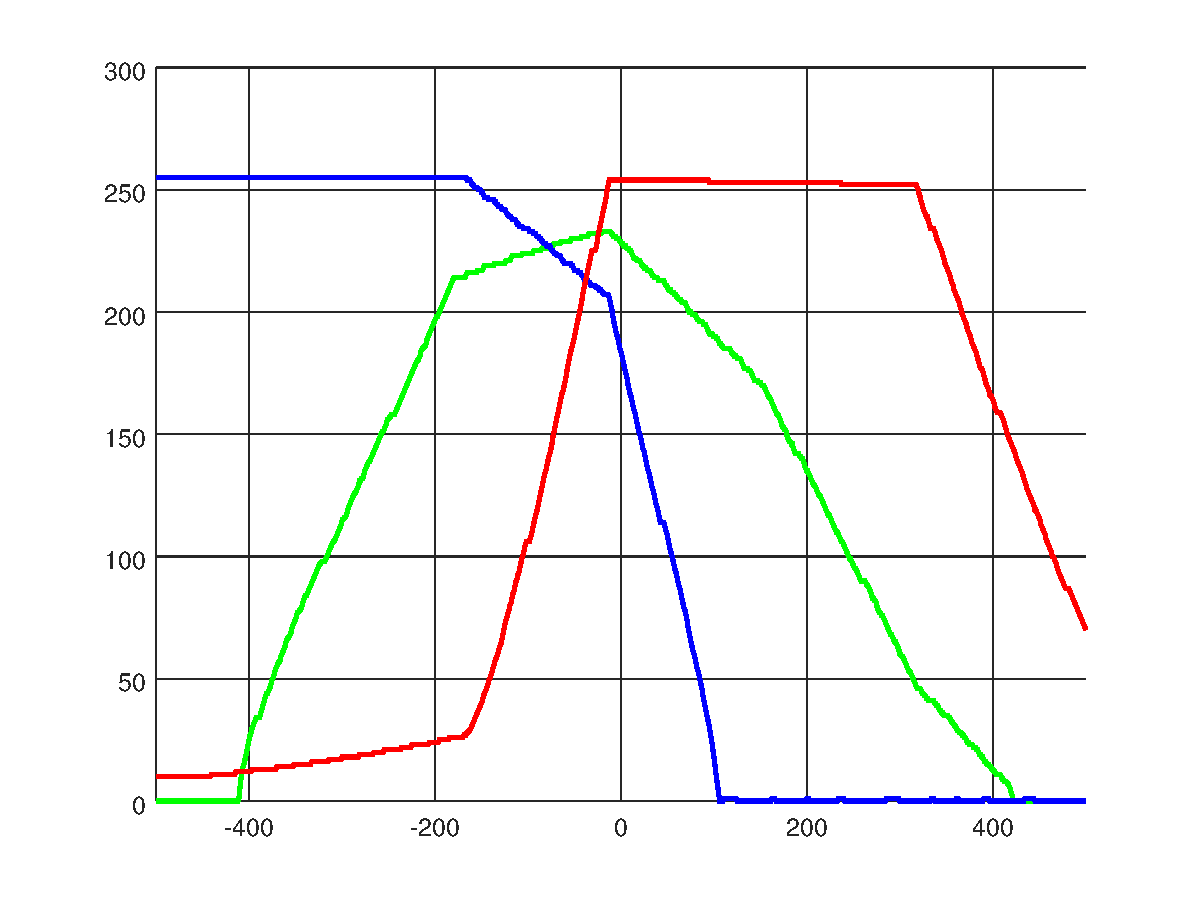
\includegraphics[width=\linewidth]{cmb/converter/rgb-graph.pdf}
	\caption{RGB Profil des in Abbildung~\ref{fig:color-strip-orig} 
		verwendeten Farbverlaufs.}
	\label{fig:color-strip-orig-rgb}
\end{figure}

\begin{figure}
	\centering
	
\includegraphics[width=\linewidth]{cmb/converter/converter-function-strip.png}
	\caption{Der für die erste Analye verwendete Farbverlauf.}
	\label{fig:color-strip}
\end{figure}

\begin{figure}
	\centering
	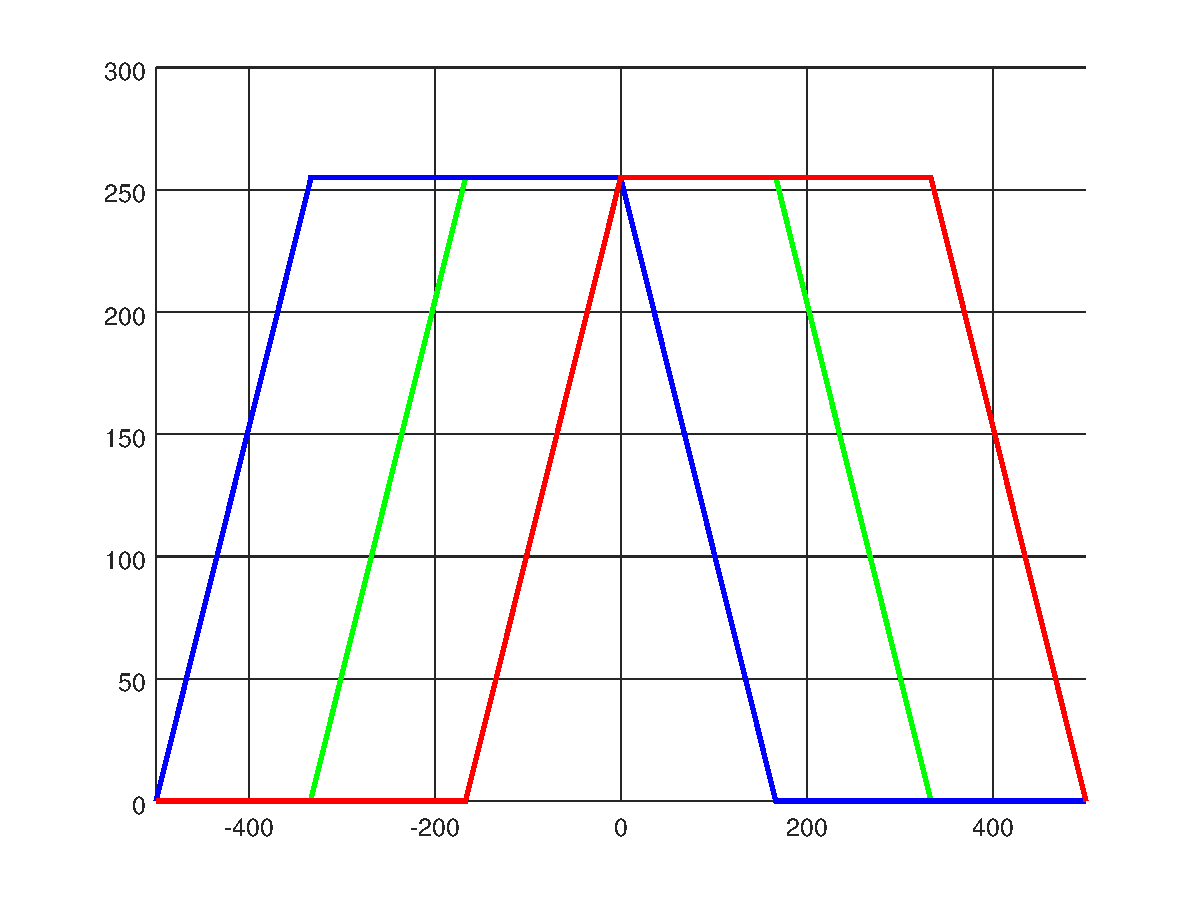
\includegraphics[width=\linewidth]{cmb/converter/converter-function.pdf}
	\caption{RGB Profil des in Abbildung~\ref{fig:color-strip} 
		verwendeten Farbverlaufs.}
	\label{fig:color-strip-rgb}
\end{figure}
% TODO: Image CMB (rectangular)
% TODO: Aufzeugung funktion der conversiation RBG -> "Kelvin"